\documentclass[twocolumn]{article}
\usepackage{epsfig}
\usepackage{xspace}
\usepackage{verbatim}


\headsep=0pt
\topmargin=0pt
\headheight=0pt
\oddsidemargin=0pt
\textwidth=6.5in
\textheight=9in
%%tth:\newcommand{\xspace}{ }
\newcommand{\fpy}{\texttt{f2py}\xspace}
\newcommand{\bs}{\symbol{`\\}}
% need bs here:
%%tth:\newcommand{\bs}{\texttt{<backslash>}}

\newcommand{\tthhide}[1]{#1}
\newcommand{\latexhide}[1]{}
%%tth:\newcommand{\tthhide}[1]{}
%%tth:\newcommand{\latexhide}[1]{#1}

\newcommand{\shell}[1]{
\latexhide{
  \special{html:
<BLOCKQUOTE>
<pre>
sh> #1
</pre>
</BLOCKQUOTE>}
}
\tthhide{
  \\[1ex]
  \hspace*{1em}
  \texttt{sh> \begin{minipage}[t]{0.8\textwidth}#1\end{minipage}}\\[1ex]
}
}

\newcommand{\email}[1]{\special{html:<A href="mailto:#1">}\texttt{<#1>}\special{html:</A>}}
\newcommand{\wwwsite}[1]{\special{html:<A href="#1">}{#1}\special{html:</A>}}
\title{Fortran to Python Interface Generator with
an Application to Aerospace Engineering}
\author{
\large Pearu Peterson\\
\small \email{pearu@cens.ioc.ee}\\
\small Center of Nonlinear Studies\\
\small Institute of Cybernetics at TTU\\
\small Akadeemia Rd 21, 12618 Tallinn, ESTONIA\\[2ex]
\large Joaquim R. R. A. Martins and Juan J. Alonso\\
\small \email{joaquim.martins@stanford.edu}, \email{jjalonso@stanford.edu}\\
\small Department of Aeronautics and Astronautics\\
\small Stanford University, CA
}
\date{$Revision: 1.17 $\\\today}
\begin{document}

\maketitle

\special{html: Other formats of this document:
<A href=f2python9.ps.gz>Gzipped PS</A>,
<A href=f2python9.pdf>PDF</A>
}

\begin{abstract}
  FPIG --- Fortran to Python Interface Generator --- is a tool for
  generating Python C/API extension modules that interface
  Fortran~77/90/95 codes with Python.  This tool automates the process
  of interface generation by scanning the Fortran source code to
  determine the signatures of Fortran routines and creating a
  Python C/API module that contains the corresponding interface
  functions.  FPIG also attempts to find dependence relations between
  the arguments of a Fortran routine call (e.g. an array and its
  dimensions) and constructs interface functions with potentially
  fewer arguments.  The tool is extremely flexible since the user has
  control over the generation process of the interface by specifying the
  desired function signatures.  The home page for FPIG can be found at
  \wwwsite{http://cens.ioc.ee/projects/f2py2e/}.

  FPIG has been used successfully to wrap a large number of Fortran
  programs and libraries.  Advances in computational science have led
  to large improvements in the modeling of physical systems which are
  often a result of the coupling of a variety of physical models that
  were typically run in isolation.  Since a majority of the available
  physical models have been previously written in Fortran, the
  importance of FPIG in accomplishing these couplings cannot be
  understated.  In this paper, we present an application of FPIG to
  create an object-oriented framework for aero-structural analysis and
  design of aircraft.
\end{abstract}

%%tth:
\tableofcontents

\section{Preface}
\label{sec:preface}

The use of high-performance computing has made it possible to tackle
many important problems and discover new physical phenomena in science
and engineering.  These accomplishments would not have been achieved
without the computer's ability to process large amounts of data in a
reasonably short time.  It can safely be said that the computer has
become an essential tool for scientists and engineers.  However, the
diversity of problems in science and engineering has left its mark as
computer programs have been developed in different programming
languages, including languages developed to describe certain specific
classes of problems.

In interdisciplinary fields it is not uncommon for scientists and
engineers to face problems that have already been solved in a
different programming environment from the one they are familiar with.
Unfortunately, researchers may not have the time or willingness to
learn a new programming language and typically end up developing the
corresponding tools in the language that they normally use.  This
approach to the development of new software can substantially impact
the time to develop and the quality of the resulting product: firstly,
it usually takes longer to develop and test a new tool than to learn a
new programming environment, and secondly it is very unlikely that a
non-specialist in a given field can produce a program that is more
efficient than more established tools.

To avoid situations such as the one described above, one alternative
would be to provide automatic or semi-automatic interfaces between programming
languages. Another possibility would be to provide language
translators, but these obviously require more work than interface
generators --- a translator must understand all language constructs
while an interface generator only needs to understand a subset of these
constructs.  With an automatic interface between two languages, scientists or
engineers can effectively use programs written in other programming
languages without ever having to learn them.

Although it is clear that it is impossible to interface arbitrary programming
languages with each other, there is no reason for doing so.  Low-level languages such as C and Fortran are well known for
their speed and are therefore suitable for applications where
performance is critical.  High-level scripting languages, on the other
hand, are generally slower but much easier to learn and use,
especially when performing interactive analysis.  Therefore, it makes
sense to create interfaces only in one direction: from lower-level
languages to higher-level languages.

In an ideal world, scientists and engineers would use higher-level
languages for the manipulation of the mathematical formulas in a problem
rather than having to struggle with tedious programming details.  For tasks
that are computationally demanding, they would use interfaces to
high-performance routines that are written in a lower-level language
optimized for execution speed.


\section{Introduction}
\label{sec:intro}

This paper presents a tool that has been developed for the creation of
interfaces between Fortran and Python.


The Fortran language is popular in
scientific computing, and is used mostly in applications that use
extensive matrix manipulations (e.g. linear algebra). Since Fortran
 has been the standard language among scientists and engineers for
 at least three decades, there is a large number of legacy codes available that
 perform a variety of tasks using very sophisticated algorithms (see
e.g. \cite{netlib}).

The Python language \cite{python}, on the other hand, is a relatively
new programming language. It is a very high-level scripting language
that supports object-oriented programming. What makes Python
especially appealing is its very clear and natural syntax, which makes it
easy to learn and use. With Python one can implement relatively
complicated algorithms and tasks in a short time with very compact
source code.

Although there are ongoing projects for extending Python's usage in
scientific computation, it lacks reliable tools that are common in
scientific and engineering such as ODE integrators, equation solvers,
tools for FEM, etc.  The implementation of all of these tools in Python
would be not only too time-consuming but also inefficient.  On the
other hand, these tools are already developed in other,
computationally more efficient languages such as Fortran or C.
Therefore, the perfect role for Python in the context of scientific
computing would be that of a ``gluing'' language.  That is, the role
of providing high-level interfaces to C, C++ and Fortran libraries.

There are a number of widely-used tools that can be used for interfacing
software libraries to Python. For binding C libraries with various
scripting languages, including Python, the tool most often used is
SWIG \cite{swig}. Wrapping Fortran routines with Python is less
popular, mainly because there are many platform and compiler-specific
issues that need to be addressed. Nevertheless, there is great
interest in interfacing Fortran libraries because they provide
invaluable tools for scientific computing. At LLNL, for example, a tool
called PyFort has been developed for connecting Fortran and
Python~\cite{pyfort}.

The tools mentioned above require an input file describing signatures
of functions to be interfaced. To create these input files, one needs
to have a good knowledge of either C or Fortran. In addition,
binding libraries that have thousands of routines can certainly constitute a
very tedious task, even with these tools.

The tool that is introduced in this paper, FPIG (Fortran to Python
Interface Generator)~\cite{fpig}, automatically generates interfaces
between Fortran and Python.  It is different from the tools mentioned
above in that FPIG can create signature files automatically by
scanning the source code of the libraries and then construct Python
C/API extension modules.  Note that the user need not be experienced
in C or even Fortran.  In addition, FPIG is designed to wrap large
Fortran libraries containing many routines with only one or two
commands.  This process is very flexible since one can always modify
the generated signature files to insert additional attributes in order
to achieve more sophisticated interface functions such as taking care
of optional arguments, predicting the sizes of array arguments and
performing various checks on the correctness of the input arguments.

The organization of this paper is as follows. First, a simple example
of FPIG usage is given. Then FPIG's basic features are described and
solutions to platform and compiler specific issues are discussed.
Unsolved problems and future work on FPIG's development are also
addressed.  Finally, an application to a large aero-structural solver
is presented as real-world example of FPIG's usage.

\section{Getting Started}
\label{sec:getstart}

To get acquainted with FPIG, let us consider the simple Fortran~77
subroutine shown in Fig. \ref{fig:exp1.f}.
\begin{figure}[htb]
  \latexhide{\label{fig:exp1.f}}
  \special{html:<BLOCKQUOTE>}
  \verbatiminput{examples/exp1.f}
  \special{html:</BLOCKQUOTE>}
  \caption{Example Fortran code \texttt{exp1.f}. This routine calculates
 the simplest rational lower and upper approximations to $e$ (for
   details of
    the algorithm see \cite{graham-etal}, p.122)}
  \tthhide{\label{fig:exp1.f}}
\end{figure}
In the sections that follow, two ways of creating interfaces to this
Fortran subroutine are described. The first and simplest way is
suitable for Fortran codes that are developed in connection with \fpy.
The second and not much more difficult method, is suitable for
interfacing existing Fortran libraries which might have been developed
by other programmers.

Numerical Python~\cite{numpy} is needed in order to compile extension
modules generated by FPIG.

\subsection{Interfacing Simple Routines}
\label{sec:example1}

In order to call the Fortran routine \texttt{exp1} from Python, let us
create an interface to it by using \fpy (FPIG's front-end program). In
order to do this, we issue the following command, \shell{f2py -m foo
exp1.f} where the option \texttt{-m foo} sets the name of the Python
C/API extension module that \fpy will create to
\texttt{foo}.  To learn more about the \fpy command line options, run \fpy
without arguments.

The output messages in Fig. \ref{fig:f2pyoutmess}
illustrate the procedure followed by \fpy:
 (i) it scans the Fortran source code specified in the command line,
 (ii) it analyses and determines the routine signatures,
 (iii) it constructs the corresponding Python C/API extension modules,
 (iv) it writes documentation to a LaTeX file, and
 (v) it creates a GNU Makefile for building the shared modules.
\begin{figure}[htb]
  \latexhide{\label{fig:f2pyoutmess}}
  \special{html:<BLOCKQUOTE>}
  {\tthhide{\small}
  \verbatiminput{examples/exp1mess.txt}
  }
  \special{html:</BLOCKQUOTE>}
  \caption{Output messages of \texttt{f2py -m foo exp1.f}.}
  \tthhide{\label{fig:f2pyoutmess}}
\end{figure}

Now we can build the \texttt{foo} module:
\shell{make -f Makefile-foo}

Figure \ref{fig:exp1session} illustrates a sample session for
 calling the Fortran routine \texttt{exp1} from Python.
\begin{figure}[htb]
  \latexhide{\label{fig:exp1session}}
  \special{html:<BLOCKQUOTE>}
  \verbatiminput{examples/exp1session.txt}
  \special{html:</BLOCKQUOTE>}
  \caption{Calling Fortran routine \texttt{exp1} from Python. Here
  \texttt{l[0]/l[1]} gives an estimate to $e$ with absolute error
    less than \texttt{u[0]/u[1]-l[0]/l[1]} (this value may depend on
    the platform and compiler used).}
  \tthhide{\label{fig:exp1session}}
\end{figure}

Note the difference between the signatures of the Fortran routine
\texttt{exp1(l,u,n)} and the corresponding wrapper function
\texttt{l,u=exp1([n])}. Clearly, the later is more informative to
the user: \texttt{exp1} takes one optional argument \texttt{n} and it
returns \texttt{l}, \texttt{u}.  This exchange of signatures is
achieved by special comment lines (starting with \texttt{Cf2py}) in
the Fortran source code --- these lines are interpreted by \fpy as
normal Fortran code.  Therefore, in the given example the line \texttt{Cf2py
  integer*4 :: n = 1} informs \fpy that the variable \texttt{n} is
optional with a default value equal to one. The line \texttt{Cf2py
  intent(out) l,u} informs \fpy that the variables \texttt{l,u} are to be
returned to Python after calling Fortran function \texttt{exp1}.

\subsection{Interfacing Libraries}
\label{sec:example2}

In our example the Fortran source \texttt{exp1.f} contains \fpy
specific information, though only as comments.  When interfacing
libraries from other parties, it is not recommended to modify their
source.  Instead, one should use a special auxiliary file to collect
the signatures of all Fortran routines and insert \fpy specific
declaration and attribute statements in that file. This auxiliary file
is called a \emph{signature file} and is identified by the extension
\texttt{.pyf}.

We can use \fpy to generate these signature files by using the
\texttt{-h <filename>.pyf} option.
In our example,  \fpy could have been called as follows,
\shell{f2py -m foo -h foo.pyf exp1.f}
where the option \texttt{-h foo.pyf} requests \fpy to read the
routine signatures, save them to the file \texttt{foo.pyf}, and then
exit.
If \texttt{exp1.f} in Fig.~\ref{fig:exp1.f} were to
contain no lines starting with \texttt{Cf2py}, the corresponding
signature file \texttt{foo.pyf} would be as shown in Fig.~\ref{fig:foo.pyf}.
In order to obtain the exchanged and more convenient signature
\texttt{l,u=foo.exp1([n])}, we would edit \texttt{foo.pyf} as shown in
Fig.~\ref{fig:foom.pyf}.
The Python C/API extension module \texttt{foo} can be constructed by
applying \fpy to the signature file with the following command:
\shell{f2py foo.pyf}
The procedure for building the corresponding shared module and using
it in Python is identical to the one described in the previous section.

\begin{figure}[htb]
  \latexhide{\label{fig:foo.pyf}}
  \special{html:<BLOCKQUOTE>}
  \verbatiminput{examples/foo.pyf}
  \special{html:</BLOCKQUOTE>}
  \caption{Raw signature file \texttt{foo.pyf} generated with
  \texttt{f2py -m foo -h foo.pyf exp1.f}}
  \tthhide{\label{fig:foo.pyf}}
\end{figure}
\begin{figure}[htb]
  \latexhide{\label{fig:foom.pyf}}
  \special{html:<BLOCKQUOTE>}
  \verbatiminput{examples/foom.pyf}
  \special{html:</BLOCKQUOTE>}
  \caption{Modified signature file \texttt{foo.pyf}}
  \tthhide{\label{fig:foom.pyf}}
\end{figure}

As we can see, the syntax of the signature file is an
extension of the Fortran~90/95 syntax. This means that only a few new
constructs are introduced for \fpy in addition to all standard Fortran
constructs; signature files can even be written in fixed form. A
complete set of constructs that are used when creating interfaces, is
described in the \fpy User's Guide \cite{f2py-ug}.


\section{Basic Features}
\label{sec:features}

In this section a short overview of \fpy features is given.
\begin{enumerate}
\item All basic Fortran types are supported. They include
the following type specifications:
\begin{verbatim}
integer[ | *1 | *2 | *4 | *8 ]
logical[ | *1 | *2 | *4 | *8 ]
real[ | *4 | *8 | *16 ]
complex[ | *8 | *16 | *32 ]
double precision, double complex
character[ |*(*)|*1|*2|*3|...]
\end{verbatim}
In addition, they can all be in the kind-selector form
(e.g. \texttt{real(kind=8)}) or char-selector form
(e.g. \texttt{character(len=5)}).
\item Arrays of all basic types are supported. Dimension
  specifications can be of form \texttt{<dimension>} or
  \texttt{<start>:<end>}. In addition, \texttt{*} and \texttt{:}
  dimension specifications can be used for input arrays.
  Dimension specifications may contain also \texttt{PARAMETER}'s.
\item The following attributes are supported:
  \begin{itemize}
  \item
  \texttt{intent(in)}: used for input-only arguments.
  \item
  \texttt{intent(inout)}: used for arguments that are changed in
  place.
  \item
  \texttt{intent(out)}: used for return arguments.
  \item
  \texttt{intent(hide)}: used for arguments to be removed from
  the signature of the Python function.
  \item
  \texttt{intent(in,out)}, \texttt{intent(inout,out)}: used for
  arguments with combined behavior.
  \item
  \texttt{dimension(<dimspec>)}
  \item
  \texttt{depend([<names>])}: used
  for arguments that depend on other arguments in \texttt{<names>}.
  \item
  \texttt{check([<C booleanexpr>])}: used for checking the
  correctness of input arguments.
  \item
  \texttt{note(<LaTeX text>)}: used for
  adding notes to the module documentation.
  \item
    \texttt{optional}, \texttt{required}
  \item
    \texttt{external}: used for call-back arguments.
  \item
  \texttt{allocatable}: used for Fortran 90/95 allocatable arrays.
  \end{itemize}
\item Using \fpy one can call arbitrary Fortran~77/90/95 subroutines
  and functions from Python, including Fortran 90/95 module routines.
\item Using \fpy one can access data in Fortran~77 COMMON blocks and
  variables in Fortran 90/95 modules, including allocatable arrays.
\item Using \fpy one can call Python functions from Fortran (call-back
  functions). \fpy supports very flexible hooks for call-back functions.
\item Wrapper functions perform the necessary type conversations for their
  arguments resulting in contiguous Numeric arrays that are suitable for
  passing to Fortran routines.
\item \fpy generates documentation strings
for \texttt{\_\_doc\_\_} attributes of the wrapper functions automatically.
\item \fpy scans Fortran codes and creates the signature
  files. It automatically detects the signatures of call-back functions,
  solves argument dependencies, decides the order of initialization of
  optional arguments, etc.
\item \fpy automatically generates GNU Makefiles for compiling Fortran
  and C codes, and linking them to a shared module.
  \fpy detects available Fortran and C compilers. The
  supported compilers include the GNU project C Compiler (gcc), Compaq
  Fortran, VAST/f90 Fortran, Absoft F77/F90, and MIPSpro 7 Compilers, etc.
  \fpy has been tested to work on the following platforms: Intel/Alpha
  Linux, HP-UX, IRIX64.
\item Finally, the complete \fpy User's Guide is available in various
  formats (ps, pdf, html, dvi). A mailing list,
  \email{f2py-users@cens.ioc.ee}, is open for support and feedback. See
  the FPIG's home page for more information \cite{fpig}.
\end{enumerate}


\section{Implementation Issues}
\label{sec:impl}

The Fortran to Python interface can be thought of as a three layer
``sandwich'' of different languages: Python, C, and Fortran.  This
arrangement has two interfaces: Python-C and C-Fortran. Since Python
itself is written in C, there are no basic difficulties in
implementing the Python-C interface~\cite{python-doc:ext}.  The C-Fortran
interface, on the other hand, results in many platform and compiler specific
issues that have to be dealt with.  We will now discuss these issues
in some detail and describe how they are solved in FPIG.

\subsection{Mapping Fortran Types to C Types}
\label{sec:mapF2Ctypes}

Table \ref{tab:mapf2c} defines how Fortran types are mapped to C types
in \fpy.
\begin{table}[htb]
  \begin{center}
    \begin{tabular}[c]{l|l}
      Fortran type & C type \\\hline
      \texttt{integer *1} & \texttt{char}\\
      \texttt{byte} & \texttt{char}\\
      \texttt{integer *2} & \texttt{short}\\
      \texttt{integer[ | *4]} & \texttt{int}\\
      \texttt{integer *8} & \texttt{long long}\\
      \texttt{logical *1} & \texttt{char}\\
      \texttt{logical *2} & \texttt{short}\\
      \texttt{logical[ | *4]} & \texttt{int}\\
      \texttt{logical *8} & \texttt{int}\\
      \texttt{real[ | *4]} & \texttt{float}\\
      \texttt{real *8} & \texttt{double}\\
      \texttt{real *16} & \texttt{long double}\\
      \texttt{complex[ | *8]} & \texttt{struct \{float r,i;\}}\\
      \texttt{complex *16} & \texttt{struct \{double r,i;\}}\\
      \texttt{complex *32} & \texttt{struct \{long double r,i;\}}\\
      \texttt{character[*...]} & \texttt{char *}\\
    \end{tabular}
    \caption{Mapping Fortran types to C types.}
    \label{tab:mapf2c}
  \end{center}
\end{table}
Users may redefine these mappings by creating a \texttt{.f2py\_f2cmap}
file in the working directory. This file should contain a Python
dictionary of dictionaries, e.g. \texttt{\{'real':\{'low':'float'\}\}},
that informs \fpy to map Fortran type \texttt{real(low)}
to C type \texttt{float} (here \texttt{PARAMETER low = ...}).


\subsection{Calling Fortran (Module) Routines}
\label{sec:callrout}

When mixing Fortran and C codes, one has to know how function names
are mapped to low-level symbols in their object files. Different
compilers may use different conventions for this purpose. For example, gcc
appends the underscore \texttt{\_} to a Fortran routine name. Other
compilers may use upper case names, prepend or append different
symbols to Fortran routine names or both. In any case, if the
low-level symbols corresponding to Fortran routines are valid for the
C language specification, compiler specific issues can be solved by
using CPP macro features.

Unfortunately, there are Fortran compilers that use symbols in
constructing low-level routine names that are not valid for C. For
example, the (IRIX64) MIPSpro 7 Compilers use `\$' character in the
low-level names of module routines which makes it impossible (at
least directly) to call such routines from C when using the MIPSpro 7
C Compiler.

In order to overcome this difficulty, FPIG introduces an unique
solution: instead of using low-level symbols for calling Fortran
module routines from C, the references to such routines are determined
at run-time by using special wrappers. These wrappers are called once
during the initialization of an extension module. They are simple
Fortran subroutines that use a Fortran module and call another C
function with Fortran module routines as arguments in order to save
their references to C global variables that are later used for calling
the corresponding Fortran module routines. This arrangement is
set up as follows. Consider the following Fortran 90 module with the
subroutine \texttt{bar}:
\special{html:<BLOCKQUOTE>}
\begin{verbatim}
module fun
  subroutine bar()
  end
end
\end{verbatim}
\special{html:</BLOCKQUOTE>}
Figure \ref{fig:capi-sketch} illustrates a Python C/API extension
module for accessing the F90 module subroutine \texttt{bar} from Python.
When the Python module \texttt{foo} is loaded, \texttt{finitbar} is
called. \texttt{finitbar} calls \texttt{init\_bar} by passing the
reference of the Fortran 90 module subroutine \texttt{bar} to C where it is
saved to the variable \texttt{bar\_ptr}. Now, when one executes \texttt{foo.bar()}
from Python, \texttt{bar\_ptr} is used in \texttt{bar\_capi} to call
the F90 module subroutine \texttt{bar}.
\begin{figure}[htb]
  \latexhide{\label{fig:capi-sketch}}
  \special{html:<BLOCKQUOTE>}
\begin{verbatim}
#include "Python.h"
...
char *bar_ptr;
void init_bar(char *bar) {
  bar_ptr = bar;
}
static PyObject *
bar_capi(PyObject *self,PyObject *args) {
  ...
  (*((void *)bar_ptr))();
  ...
}
static PyMethodDef
foo_module_methods[] = {
  {"bar",bar_capi,METH_VARARGS},
  {NULL,NULL}
};
extern void finitbar_; /* GCC convention */
void initfoo() {
  ...
  finitbar_(init_bar);
  Py_InitModule("foo",foo_module_methods);
  ...
}
\end{verbatim}
  \special{html:</BLOCKQUOTE>}
  \caption{Sketch of Python C/API for accessing F90 module subroutine
    \texttt{bar}. The Fortran function \texttt{finitbar} is defined in
  Fig.~\ref{fig:wrapbar}.}
  \tthhide{\label{fig:capi-sketch}}
\end{figure}
\begin{figure}[ht]
  \latexhide{\label{fig:wrapbar}}
\special{html:<BLOCKQUOTE>}
\begin{verbatim}
      subroutine finitbar(cinit)
        use fun
        extern cinit
        call cinit(bar)
      end
\end{verbatim}
\special{html:</BLOCKQUOTE>}
  \caption{Wrapper for passing the reference of \texttt{bar} to C code.}
  \tthhide{\label{fig:wrapbar}}
\end{figure}

Surprisingly, mixing C code and Fortran modules in this way is as
portable and compiler independent as mixing C and ordinary Fortran~77
code.

Note that extension modules generated by \fpy actually use
\texttt{PyFortranObject} that implements above described scheme with
exchanged functionalities (see Section \ref{sec:PFO}).


\subsection{Wrapping Fortran Functions}
\label{sec:wrapfunc}

The Fortran language has two types of routines: subroutines and
functions. When a Fortran function returns a composed type such as
\texttt{COMPLEX} or \texttt{CHARACTER}-array then calling this
function directly from C may not work for all compilers, as C
functions are not supposed to return such references. In order to
avoid this, FPIG constructs an additional Fortran wrapper subroutine
for each such Fortran function. These wrappers call just the
corresponding functions in the Fortran layer and return the result to
C through its first argument.


\subsection{Accessing Fortran Data}
\label{sec:accsdata}

In Fortran one can use \texttt{COMMON} blocks and Fortran module
variables to save data that is accessible from other routines.  Using
FPIG, one can also access these data containers from Python. To achieve
this, FPIG uses special wrapper functions (similar to the ones used
for wrapping Fortran module routines) to save the references to these
data containers so that they can later be used from C.

FPIG can also handle \texttt{allocatable} arrays. For example, if a
Fortran array is not yet allocated, then by assigning it in Python,
the Fortran to Python interface will allocate and initialize the
array.  For example, the F90 module allocatable array \texttt{bar}
defined in
\special{html:<BLOCKQUOTE>}
\begin{verbatim}
module fun
  integer, allocatable :: bar(:)
end module
\end{verbatim}
\special{html:</BLOCKQUOTE>}
can be allocated from Python as follows
\special{html:<BLOCKQUOTE>}
\begin{verbatim}
>>> import foo
>>> foo.fun.bar = [1,2,3,4]
\end{verbatim}
\special{html:</BLOCKQUOTE>}

\subsection{\texttt{PyFortranObject}}
\label{sec:PFO}

In general, we would like to access from Python the following Fortran
objects:
\begin{itemize}
\item subroutines and functions,
\item F90 module subroutines and functions,
\item items in COMMON blocks,
\item F90 module data.
\end{itemize}
Assuming that the Fortran source is available, we can determine the signatures
of these objects (the full specification of routine arguments, the
layout of Fortran data, etc.).  In fact, \fpy gets this information
while scanning the Fortran source.

In order to access these Fortran objects from C, we need to determine
their references. Note that the direct access of F90 module objects is
extremely compiler dependent and in some cases even impossible.
Therefore, FPIG uses various wrapper functions for obtaining the
references to Fortran objects. These wrapper functions are ordinary
F77 subroutines that can easily access objects from F90 modules and
that pass the references to Fortran objects as C variables.


\fpy generated Python C/API extension modules use
\texttt{PyFortranObject} to store the references of Fortran objects.
In addition to the storing functionality, the \texttt{PyFortranObject}
also provides methods for accessing/calling Fortran objects from
Python in a user-friendly manner. For example, the item \texttt{a} in
\texttt{COMMON /bar/ a(2)} can be accessed from Python as
\texttt{foo.bar.a}.

Detailed examples of \texttt{PyFortranObject} usage can be found in
\cite{PFO}.

\subsection{Callback Functions}
\label{sec:callback}

Fortran routines may have arguments specified as \texttt{external}.
These arguments are functions or subroutines names that the receiving Fortran routine
will call from its body. For such arguments FPIG
constructs a call-back mechanism (originally contributed by Travis
Oliphant) that allows Fortran routines to call Python functions. This
is actually realized using a C layer between Python and
Fortran. Currently, the call-back mechanism is compiler independent
unless a call-back function needs to return a composed type
(e.g. \texttt{COMPLEX}).

The signatures of call-back functions are determined when \fpy scans
the Fortran source code. To illustrate this, consider the following
example:
\special{html:<BLOCKQUOTE>}
\begin{verbatim}
      subroutine foo(bar, fun, boo)
        integer i
        real r
        external bar,fun,boo
        call bar(i, 1.2)
        r = fun()
        call sun(boo)
      end
\end{verbatim}
\special{html:</BLOCKQUOTE>}
\fpy recognizes the signatures of the user routines \texttt{bar} and
\texttt{fun} using the information contained in the lines \texttt{call
  bar(i, 1.2)} and \texttt{r = fun()}:
\special{html:<BLOCKQUOTE>}
\begin{verbatim}
subroutine bar(a,b)
  integer a
  real b
end
function fun()
  real fun
end
\end{verbatim}
\special{html:</BLOCKQUOTE>}
But \fpy cannot determine the signature of the user routine
\texttt{boo} because the source contains no information at all about
the \texttt{boo} specification. Here user needs to provide the
signature of \texttt{boo} manually.

\section{Future Work}
\label{sec:future}

FPIG can be used to wrap almost any Fortran code. However, there are
still issues that need to be resolved. Some of them are listed below:
\begin{enumerate}
\item One of the FPIG's goals is to become as platform and compiler
  independent as possible. Currently FPIG can be used on
  any UN*X platform that has gcc installed in it. In the future, FPIG
  should be also tested on Windows systems.
\item Another goal of FPIG is to become as simple to use as
  possible. To achieve that, FPIG should start using the facilities of
  \texttt{distutils}, the new Python standard to distribute and build
  Python modules. Therefore, a contribution to \texttt{distutils}
  that can handle Fortran extensions should be developed.
\item Currently users must be aware of
  the fact that multi-dimensional arrays are stored differently in C
  and Fortran (they must provide transposed multi-dimensional arrays
  to wrapper functions). In the future a solution should be found such
  that users do not need to worry about this rather
  confusing and technical detail.
\item Finally, a repository of signature files for widely-used Fortran
  libraries (e.g. BLAS, LAPACK, MINPACK, ODEPACK, EISPACK, LINPACK) should be
  provided.
\end{enumerate}


\section{Application to a Large Aero-Structural Analysis Framework}
\label{sec:app}


\subsection{The Need for Python and FPIG}
\label{sec:appsub1}

As a demonstration of the power and usefulness of FPIG, we will
present work that has been done at the Aerospace Computing Laboratory
at Stanford University. The focus of the research is on aircraft
design optimization using high-fidelity analysis tools such as
Computational Fluid Dynamics (CFD) and Computational Structural
Mechanics (CSM)~\cite{reno99}.

The group's analysis programs are written mainly in Fortran and are the result
of many years of development.  Until now, any researcher that needed
to use these tools would have to learn a less than user-friendly
interface and become relatively familiar with the inner workings of
the codes before starting the research itself.  The need to
couple analyses of different disciplines revealed the additional
inconvenience of gluing and scripting the different codes with
Fortran.

It was therefore decided that the existing tools should be wrapped
using an object-oriented language in order to improve their ease of
use and versatility.  The use of several different languages such as
C++, Java and Perl was investigated but Python seemed to provide the
best solution. The fact that it combines scripting capability
with a fully-featured object-oriented programming language, and that
it has a clean syntax were factors that determined our choice. The
introduction of tools that greatly facilitate the task of wrapping
Fortran with Python provided the final piece needed to realize our
objective.

\subsection{Wrapping the Fortran Programs}

In theory, it would have been possible to wrap our Fortran programs
with C and then with Python by hand.  However, this would have been a
labor intensive task that would detract from our research.  The use of
tools that automate the task of wrapping has been extremely useful.

The first such tool that we used was PyFort.  This tool created the C
wrappers and Python modules automatically, based on signature files
(\texttt{.pyf}) provided by the user.  Although it made the task of
wrapping considerably easier, PyFort was limited by the fact that any
Fortran data that was needed at the Python level had to be passed in
the argument list of the Fortran subroutine.  Since the bulk of the
data in our programs is shared by using Fortran~77 common blocks and
Fortran~90 modules, this required adding many more arguments to the
subroutine headers.  Furthermore, since Fortran does not allow common
block variables or module data to be specified in a subroutine
argument list, a dummy pointer for each desired variable had to be
created and initialized.

The search for a better solution to this problem led us to \fpy.
Since \fpy provides a solution for accessing common block and module
variables, there was no need to change the Fortran source anymore,
making the wrapping process even easier.  With \fpy we also
experienced an increased level of automation since it produces the
signature files automatically, as well as a Makefile for the joint
compilation of the original Fortran and C wrapper codes. This increased
automation did not detract from its flexibility since it was always
possible to edit the signature files to provide different functionality.

Once Python interfaces were created for each Fortran application
by running \fpy, it was just a matter of using Python to achieve the
final objective of developing an object-oriented framework for our
multidisciplinary solvers. The Python modules that we designed are
discussed in the following section.


\subsection{Module Design}
\label{ssec:module}

The first objective of this effort was to design the classes for each
type of analysis, each representing an independent Python module. In
our case, we are interested in performing aero-structural analysis and
optimization of aircraft wings. We therefore needed an analysis tool
for the flow (CFD), another for analyzing the structure (CSM), as well
as a geometry database. In addition, we needed to interface these two
tools in order to analyze the coupled system. The object design for
each of these modules should be general enough that the underlying
analysis code in Fortran can be changed without changing the Python
interface.  Another requirement was that the modules be usable on
their own for single discipline analysis.

\subsubsection{Geometry}

The \emph{Geometry} class provides a database for the outer mold
geometry of the aircraft.  This database needs to be accessed by both
the flow and structural solvers.  It contains a parametric description
of the aircraft's surface as well as methods that extract and update
this information.


\subsubsection{Flow}

The flow solver was wrapped in a class called \emph{Flow}. The class
was designed so that it can wrap any type of CFD solver. It contains
two main objects: the computational mesh and a solver object. A graph
showing the hierarchy of the objects in \emph{Flow} is shown in
Fig.~\ref{fig:flow}.
\tthhide{
\begin{figure}[h]
  \centering
  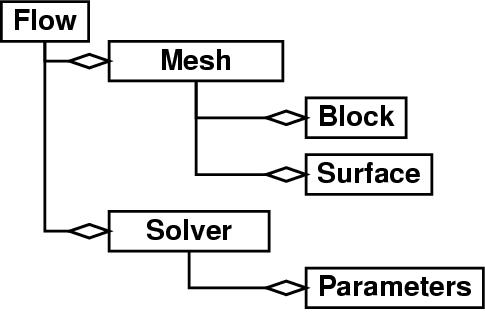
\epsfig{file=./flow.eps, angle=0, width=.7\linewidth}
  \caption{The \emph{Flow} container class.}
  \label{fig:flow}
\end{figure}
}
\latexhide{
\begin{figure}[h]
  \label{fig:flow}
\special{html:
<CENTER>
 <IMG SRC="flow.jpg" WIDTH="400">
</CENTER>
}
  \caption{The \emph{Flow} container class.}
\end{figure}
}
Methods in the flow class include those used for the initialization of
all the class components as well as methods that write the current
solution to a file.


\subsubsection{Structure}

The \emph{Structure} class wraps a structural analysis code. The class
stores the information about the structure itself in an object called
\emph{Model} which also provides methods for changing and exporting
its information. A list of the objects contained in this class can be
seen in Fig.~\ref{fig:structure}.
\tthhide{
\begin{figure}[h]
  \centering
  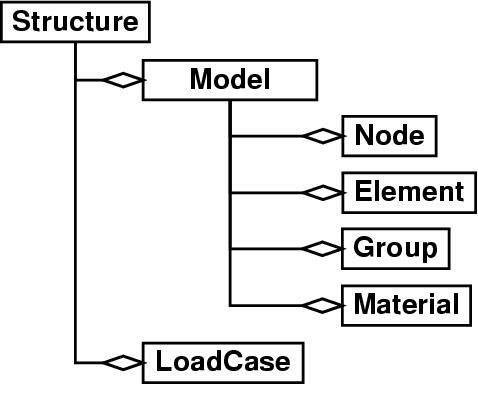
\epsfig{file=./structure.eps, angle=0, width=.7\linewidth}
  \caption{The \emph{Structure} container class.}
  \label{fig:structure}
\end{figure}
}
\latexhide{
\begin{figure}[h]
  \label{fig:structure}
\special{html:
<CENTER>
 <IMG SRC="structure.jpg" WIDTH="400">
</CENTER>
}
  \caption{The \emph{Structure} container class.}
\end{figure}
}
Since the \emph{Structure} class contains a
dictionary of \emph{LoadCase} objects, it is able to store and solve
multiple load cases, a capability that the original Fortran code
does not have.


\subsubsection{Aerostructure}

The \emph{Aerostructure} class is the main class in the
aero-structural analysis module and contains a \emph{Geometry}, a
\emph{Flow} and a \emph{Structure}.  In addition, the class defines
all the functions that are necessary to translate aerodynamic
loads to structural loads and structural displacements to
geometry surface deformations.

One of the main methods of this class is the one that solves the
aeroelastic system. This method is printed below:
\begin{verbatim}
def Iterate(self, load_case):
  """Iterates the aero-structural solution."""
  self.flow.Iterate()
  self._UpdateStructuralLoads()
  self.structure.CalcDisplacements(load_case)
  self.structure.CalcStresses(load_case)
  self._UpdateFlowMesh()
  return
\end{verbatim}
This is indeed a very readable script, thanks to Python, and any
high-level changes to the solution procedure can be easily
implemented.
The \emph{Aerostructure} class also contains methods that export all
the information on the current solution for visualization, an example
of which is shown in the next section.


\subsection{Results}

In order to visualize results, and because we needed to view results
from multiple disciplines simultaneously, we selected OpenDX. Output
files in DX format are written at the Python level and the result can
be seen in Fig.~\ref{fig:aerostructure} for the case of a transonic
airliner configuration.
\tthhide{
\begin{figure*}[t]
  \centering
  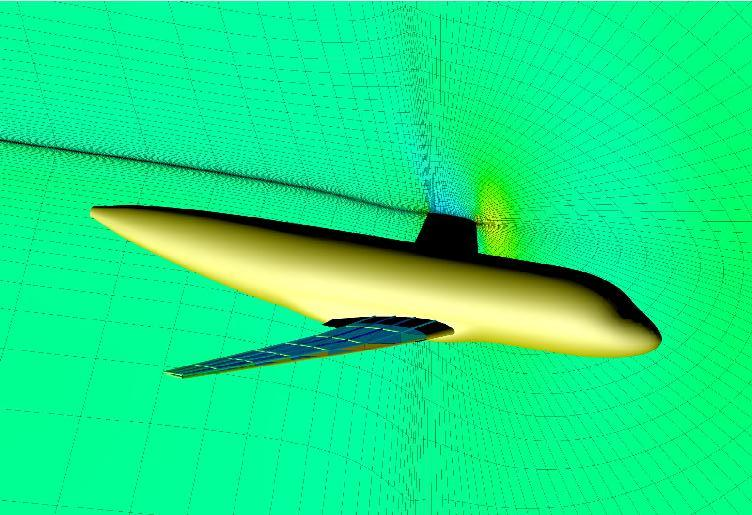
\epsfig{file=./aerostructure.eps, angle=-90, width=\linewidth}
  \caption{Aero-structural model and results.}
  \label{fig:aerostructure}
\end{figure*}
}
\latexhide{
\begin{figure}[h]
  \label{fig:aerostructure}
\special{html:
<CENTER>
 <IMG SRC="aerostructure.jpg" WIDTH="600">
</CENTER>
}
  \caption{Aero-structural model and results.}
\end{figure}
}


The figure illustrates the multidisciplinary nature of the
problem. The grid pictured in the background is the mesh used by the
flow solver and is colored by the pressure values computed at the
cell centers. The wing in the foreground and its outer surface is
clipped to show the internal structural components which are colored
by their stress value.

In conclusion, \fpy and Python have been extremely useful tools in our
pursuit for increasing the usability and flexibility of existing Fortran
tools.


\begin{thebibliography}{99}
\bibitem{netlib}
\newblock Netlib repository at UTK and ORNL.
\newblock \\\wwwsite{http://www.netlib.org/}
\bibitem{python}
Python language.
\newblock \\\wwwsite{http://www.python.org/}
\bibitem{swig}
SWIG --- Simplified Wrapper and Interface Generator.
\newblock \\\wwwsite{http://www.swig.org/}
\bibitem{pyfort}
PyFort --- The Python-Fortran connection tool.
\newblock \\\wwwsite{http://pyfortran.sourceforge.net/}
\bibitem{fpig}
FPIG --- Fortran to Python Interface Generator.
\newblock \\\wwwsite{http://cens.ioc.ee/projects/f2py2e/}
\bibitem{numpy}
Numerical Extension to Python.
\newblock \\\wwwsite{http://numpy.sourceforge.net/}
\bibitem{graham-etal}
R. L. Graham, D. E. Knuth, and O. Patashnik.
\newblock {\em {C}oncrete {M}athematics: a foundation for computer science.}
\newblock Addison-Wesley, 1988
\bibitem{f2py-ug}
P. Peterson.
\newblock {\em {\tt f2py} - Fortran to Python Interface Generator. Second Edition.}
\newblock 2000
\newblock
\\\wwwsite{http://cens.ioc.ee/projects/f2py2e/usersguide.html}
\bibitem{python-doc:ext}
Python Documentation: Extending and Embedding.
\newblock \\\wwwsite{http://www.python.org/doc/ext/}
\bibitem{PFO}
P. Peterson. {\em {\tt PyFortranObject} example usages.}
\newblock 2001
\newblock \\\wwwsite{http://cens.ioc.ee/projects/f2py2e/pyfobj.html}
\bibitem{reno99}
Reuther, J., J. J. Alonso, J. R. R. A. Martins, and
S. C. Smith.
\newblock ``A Coupled Aero-Structural Optimization Method for
  Complete Aircraft Configurations'',
\newblock {\em Proceedings of the 37th Aerospace Sciences Meeting},
\newblock AIAA Paper 1999-0187. Reno, NV, January, 1999
\end{thebibliography}

%\end{multicols}

%\begin{figure}[htbp]
%  \begin{center}
%    \epsfig{file=aerostructure2b.ps,width=0.75\textwidth}
%  \end{center}
%\end{figure}



\end{document}

%%% Local Variables:
%%% mode: latex
%%% TeX-master: t
%%% End:
